% A skeleton file for producing Computer Engineering reports
% https://kgcoe-git.rit.edu/jgm6496/KGCOEReport_template

\documentclass[CMPE]{../KGCOEReport}

% The following should be changed to represent your personal information
\newcommand{\classCode}{CMPE 460}  % 4 char code with number
\newcommand{\name}{Andrei Tumbar}
\newcommand{\LabSectionNum}{2}
\newcommand{\LabInstructor}{Beato}
\newcommand{\TAs}{Xavier Brooks\\
Diana Yakobchuk}
\newcommand{\LectureSectionNum}{1}
\newcommand{\LectureInstructor}{Beato}
\newcommand{\exerciseNumber}{3}
\newcommand{\exerciseDescription}{Characterization of OPB745}
\newcommand{\dateDone}{January 27th}
\newcommand{\dateSubmitted}{February 4th}

\usepackage{tikz}
\usepackage{circuitikz}
\usetikzlibrary{calc}
\usetikzlibrary{circuits.logic.IEC,calc}
\usepackage{multirow}
\usepackage{float}
\usepackage{lmodern}
\usepackage{siunitx}
\usepackage{subcaption}
\usepackage{graphicx}
\usepackage[usestackEOL]{stackengine}
\usepackage{scalerel}
\usepackage[T1]{fontenc}
\usepackage{amsmath}
\usepackage{pdfpages}

\ctikzset{logic ports=ieee}

\def\lbar#1{\ThisStyle{%
    \setbox0=\hbox{$\SavedStyle#1$}%
    \stackengine{2.2\LMpt}{$\SavedStyle#1$}{\rule{\wd0}{0.1\LMpt}}{O}{c}{F}{F}{S}%
}}

\DeclareFontFamily{U}{mathx}{\hyphenchar\font45}
\DeclareFontShape{U}{mathx}{m}{n}{ <-> mathx10 }{}
\DeclareSymbolFont{mathx}{U}{mathx}{m}{n}
\DeclareFontSubstitution{U}{mathx}{m}{n}
\DeclareMathAccent{\widebar}{\mathalpha}{mathx}{"73}

\makeatletter
\newcommand{\cwidebar}[2][0]{{\mathpalette\@cwidebar{{#1}{#2}}}}
\newcommand{\@cwidebar}[2]{\@cwideb@r{#1}#2}
\newcommand{\@cwideb@r}[3]{%
    \sbox\z@{$\m@th\mkern-#2mu#3\mkern#2mu$}%
    \widebar{\box\z@}%
}
\newcommand\currentcoordinate{\the\tikz@lastxsaved,\the\tikz@lastysaved}
\makeatother

\newcommand\decbin[9]{%
    \par\smallskip
    \makebox[3cm][r]{$#1$\ }\fbox{#2}\,\fbox{#3}\,\fbox{#4}\,\fbox{#5}\,\fbox{#6}\,\fbox{#7}\,\fbox{#8}\,\fbox{#9}\par}


\def\code#1{\texttt{#1}}

\ctikzset{resistors/scale=0.8}

\ctikzset{logic ports/scale=0.7}

\begin{document}
    \maketitle
    \section*{Abstract}

    In this laboratory exercise, the electrical properties of the OPB745 optoisolator
    sensor was investigated. An isolation chamber with varying length was constructed
    to measure the resistivity properties of the sensor. The sensors characteristics
    were charted and compared to the device characteristic on the corresponding data
    sheet. A square wave power signal was also tested with this circuit to determine
    the frequency at which the output would degrade.

    \section*{Design Methodology}

	When designing an environment to isolate the optoisolator sensor, the most important
	design consideration is to avoid leakage of as much light as possible. To accomplish 
	this, two PVC pipes were used. One pipe has the same outer diameter as the others
	inner diameter. This allows as much light to be blocked from entering in the space
	between the two pipes.\\

	The OPB745 sensor is a set of two different diodes, a light source and its
	corresponding light detector. The basic idea is that the light source would emit
	outward and reflect off of some surface. When the light travels back to the receiver,
	the receiver diode will draw more current which allows us to measure the voltage
	drop across a series resistor. This measured voltage will give us information about
	the distance between the emitter and the reflective surface and can therefore be used
	as a distance measurement sensor.

    \subsection*{Part 1}
    
    In the first portion of this exercise the OPB745 was used to measure certain distances
    inside the isolation chamber. The voltage drop across a specific resistor was used
    to determine the current draw through the receiver which could later be used to
    chart the characteristics of the sensor output.\\

	The schematic diagram below was made to better illustrate the functionality of the
	optoisolator circuit.
    
    \begin{figure}[h!]
        \centering
        %! suppress = Ellipsis
        \begin{circuitikz}[american, ]

            \draw (0,5) to[battery, l_=5V] (0,0);
            \draw (0,5)
            		-| (2,5) to[R, l_=\(R_F\)] (2,3)
            		to[led] (2,0) -| (0,0)
            ;
            \draw (2,5) -| (4,5) to[R, l_=\(R_L\)] (4,3)
            	node[npn,photo, anchor=C](rec){}
            	(rec.E) node[npn,anchor=B](recN){}
            	(recN.C) |- (rec.C)
            	(recN.E) |- (2,0)
            ;
            \draw (rec.C -| recN.C) -- ++(1,0) coordinate(voutp);
            \draw (4,0) coordinate(voutnoff) -- (voutp |- voutnoff) coordinate(voutn)
            	(voutp) to[open,v=$V_{out}$] (voutn)
            	node[ground]{};

        \end{circuitikz}
        \caption{Part 1 schematic of optoisolator circuit}
        \label{fig:part1}
    \end{figure}
    
    Figure \ref{fig:part1} shows the circuit that was constructed in the first portion
    of the lab. Here we can see two resistors, $R_F$ and $R_L$. The load resistor $R_L$
    has known values. For the purposes of this lab, \SI{10}{\kilo\ohm} and
    \SI{20}{\kilo\ohm} were used for $R_L$. $R_F$ has an unknown resistance value dependent
    on the value of the load resistor. When determining which resistance to use for $R_F$,
    we must consider that we want the maximum allowed current to pass through the
    diode in series with $R_F$. This current is listed on the diode's data sheet at
    \SI{40}{\milli\ampere}. Using this information, the resistance of $R_F$ was determined
    to be \SI{82.5}{\ohm} and \SI{65}{\ohm} when the $R_L$ values are \SI{10}{\kilo\ohm}
    and \SI{20}{\kilo\ohm} respectively.\\

    Measurements of the sensor can be made by placing a multimeter on the $V_{out}$ node
    to measure the voltage drop on $R_L$. This information will tell us the current that
    the receiver NPN transistor was able to pass due to the amount of light it was exposed
    to.

    \subsection*{Part 2}
	
	During the second portion of this exercise, a square wave generator was used to
	pulse the current across the emitter diode and generate a square wave output signal.
	A schematic showing how the part 2 circuit differs from the part 1 circuit is shown
	below.

	\begin{figure}[h!]
        \centering
        \begin{circuitikz}

            \draw (0,5) to[battery, l_=5V] (0,0);
            \draw (0,5)
            		-| (4,5) to[R, l_=\(R_F\)] ++(0,-2)
            		to[led] ++(0,-1)
            		-- ++(-0.5,0) node[not port, anchor=out, label=7406](inv1){}
            		(inv1.in) -| ++(-0.5,-0.5) to[sqV] ++(0,-1) |- (0,0)
            		node[ground](g){}
            ;
            \draw (4,5) -| (6,5) to[R, l_=\(R_L\)] ++(0,-2)
            	node[npn,photo, anchor=C](rec){}
            	(rec.E) node[npn,anchor=B](recN){}
            	(recN.C) |- (rec.C)
            	(recN.E) |- (g)
            ;
            \draw (rec.C -| recN.C) -- ++(1,0)
            	node[not port, anchor=in, label=74LS14](inv2){}
            	(inv2.out) -- ++(1,0) node[label=$V_{out}$]{}
        	;

        \end{circuitikz}
        \caption{Part 2 schematic of optoisolator circuit with wave generator}
        \label{fig:part2}
    \end{figure}

	Figure \ref{fig:part1} and \ref{fig:part2} are both quite similar in their basic
	design. There are some new components added in series with the emission diode.
	The wave generator's purpose is to feed a period square with to the 7406 inverter.
	This inverter is not simply a logical inverter. On input level low, instead of the
	inverter outputting a logic level high, it actually provides high impedance on the
	output line. This is important because the emission diode can be damaged if a reverse
	voltage is applied to it. The result of feeding the square wave and inverter signal
	into the output of the diode is to pulse the emitter at the frequency of the square
	wave.\\

	The final 74LS14 inverter has the purpose of re-inverting the generated wave
	from the input square wave. The needs to be done because a current will only
	pass $R_L$ when the emission diode is not at high impedance. This state will only
	occur when the input from the square wave is high. When current passes through the
	$R_L$ resistor, the voltage at $V_{out}$ will be low and therefore needs to be
	inverted. The other purpose this inverter serves is to convert an analog voltage
	to a digital one. The value of the output will be floored to logic levels low and high.

    \section*{Results \& Analysis}

	To graph the characteristics of the optoisolator circuit, a table of volage readings
	is created by reading the voltage at $V_{out}$ after altering the length of
	the space between the inner and outer tubes. The same process was applied for both
	\SI{10}{\kilo\ohm} and \SI{20}{\kilo\ohm} values for the load resistor $R_L$.
	The current through the load resistor was also calculated using the voltage drop
	across the load resistor. A table of voltage measurements at $V_{out}$ was created for
	varying distances from \SI{0}{\milli\metre}-\SI{50}{\milli\metre} within the isolation
	chamber.

	\begin{table}[H]
        \renewcommand{\arraystretch}{1.2}
        \setlength{\tabcolsep}{12pt}
        \caption{Part 1 voltage readings for \SI{0}{\milli\metre}-\SI{50}{\milli\metre} for $R_L$ at \SI{10}{\kilo\ohm} and \SI{20}{\kilo\ohm}}
        \begin{center}
            \begin{tabular}{|c|c|c||c|c|}
                \hline
				$R_L$ & \multicolumn{2}{c||}{\SI{10}{\kilo\ohm}} & \multicolumn{2}{c|}{\SI{20}{\kilo\ohm}}\\\hline
				Distance (mm) & $V_{out}$ & $I_{R_L}$ (mA) & $V_{out}$ & $I_{R_L}$ (mA)\\\hline

0	& 4.25	& 0.075		& 4.945	& 0.00275\\\hline
1	& 0.683	& 0.4317	& 0.652	& 0.2174\\\hline
2	& 0.677	& 0.4323	& 0.653	& 0.21735\\\hline
3	& 0.685	& 0.4315	& 0.668	& 0.2166\\\hline
4	& 0.688	& 0.4312	& 0.689	& 0.21555\\\hline
5	& 0.707	& 0.4293	& 0.704	& 0.2148\\\hline
6	& 0.723	& 0.4277	& 0.721	& 0.21395\\\hline
7	& 0.736	& 0.4264	& 0.737	& 0.21315\\\hline
8	& 0.75	& 0.425		& 0.75	& 0.2125\\\hline
9	& 0.766	& 0.4234	& 0.761	& 0.21195\\\hline
10	& 0.801	& 0.4199	& 0.773	& 0.21135\\\hline
11	& 0.82	& 0.418		& 0.784	& 0.2108\\\hline
12	& 0.839	& 0.4161	& 0.789	& 0.21055\\\hline
13	& 0.878	& 0.4122	& 0.799	& 0.21005\\\hline
14	& 1.345	& 0.3655	& 0.809	& 0.20955\\\hline
15	& 1.671	& 0.3329	& 0.819	& 0.20905\\\hline
20	& 2.777	& 0.2223	& 1.248	& 0.1876\\\hline
25	& 3.366	& 0.1634	& 2.534	& 0.1233\\\hline
30	& 3.835	& 0.1165	& 3.321	& 0.08395\\\hline
40	& 4.447	& 0.0553	& 3.813	& 0.05935\\\hline
45	& 4.575	& 0.0425	& 4.086	& 0.0457\\\hline
50	& 4.614	& 0.0386	& 4.169	& 0.04155\\\hline

            \end{tabular}
        \end{center}
        \label{tab:p1}
    \end{table}

	Using the values from Table \ref{tab:p1}, voltage and current graph were generated
	to show the effect of distance in the inner tube on the sensor. Both graphs for $R_L$
	at \SI{10}{\kilo\ohm} and \SI{20}{\kilo\ohm} were charted alongside each other to
	compare varying load resistances.

	\begin{figure}[h!]
        \centering
        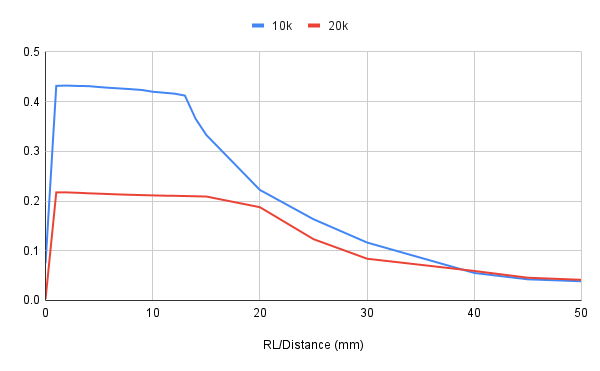
\includegraphics[width=12cm]{irl}
        \caption{$I_{R_L}$ (mA) vs distance inside isolation chamber.}
        \label{fig:irl}
	\end{figure}

	\begin{figure}[h!]
        \centering
        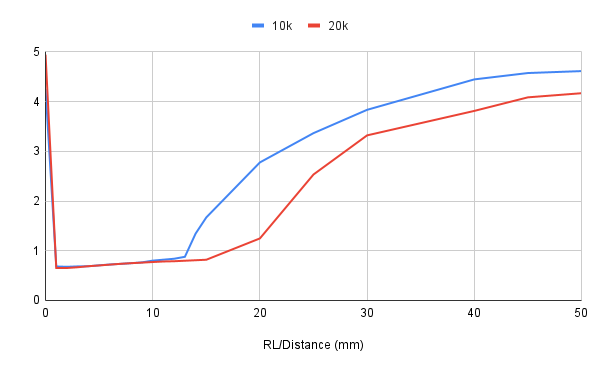
\includegraphics[width=12cm]{vout}
        \caption{Voltage at $V_{out}$ vs distance inside isolation chamber.}
        \label{fig:vout}
	\end{figure}

	Looking at figures \ref{fig:irl} and \ref{fig:vout} we can see the expected
	characteristic curves of the OPB745. The current draw should be zero when the
	distance from the sensor is zero because most of the light emitting from the
	diode does not reach the transducer on the receiving end.

	\pagebreak

	\subsection*{Part 2}

	Part 2 of the exercise involved running the second circuit at both values of $R_L$.
	The frequency input on the square wave generator was varied until the signal
	degraded.

	\begin{figure}[ht]
	\begin{subfigure}{.5\textwidth}
	  \centering
	  % include first image
	  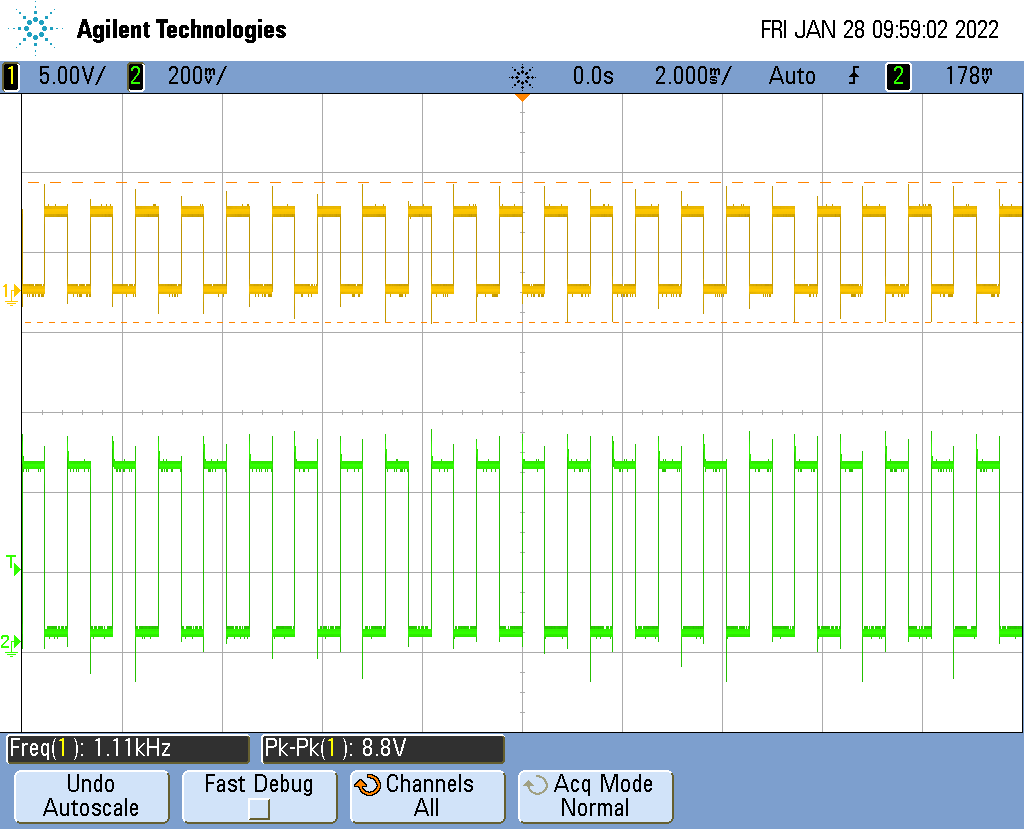
\includegraphics[width=.8\linewidth]{p700_10k}
	  \caption{Signal at \SI{700}{\hertz}}
	  \label{fig:sub-first}
	\end{subfigure}
	\begin{subfigure}{.5\textwidth}
	  \centering
	  % include second image
	  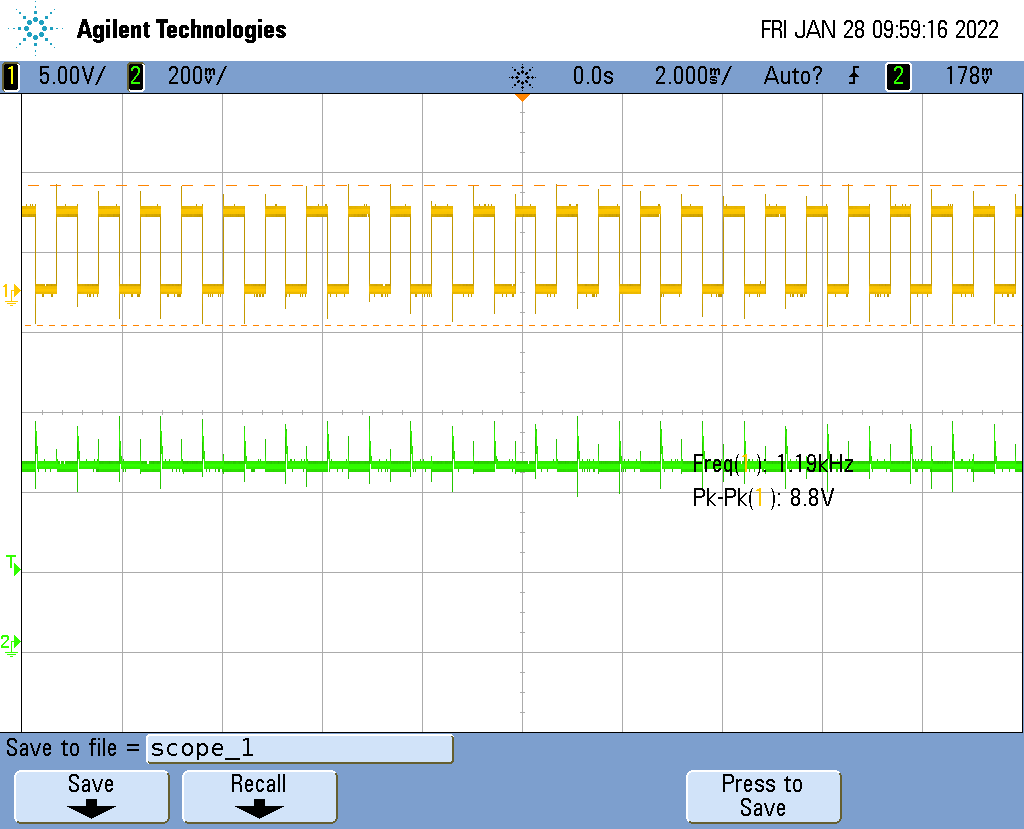
\includegraphics[width=.8\linewidth]{p800_10k}
	  \caption{Degraded signal at \SI{800}{\hertz}}
	  \label{fig:sub-second}
	\end{subfigure}
	\caption{Screen captures of oscilloscope with $R_L=\SI{10}{\kilo\ohm}$}
	\label{fig:p21}
	\end{figure}

	\begin{figure}[ht]
	\begin{subfigure}{.5\textwidth}
	  \centering
	  % include first image
	  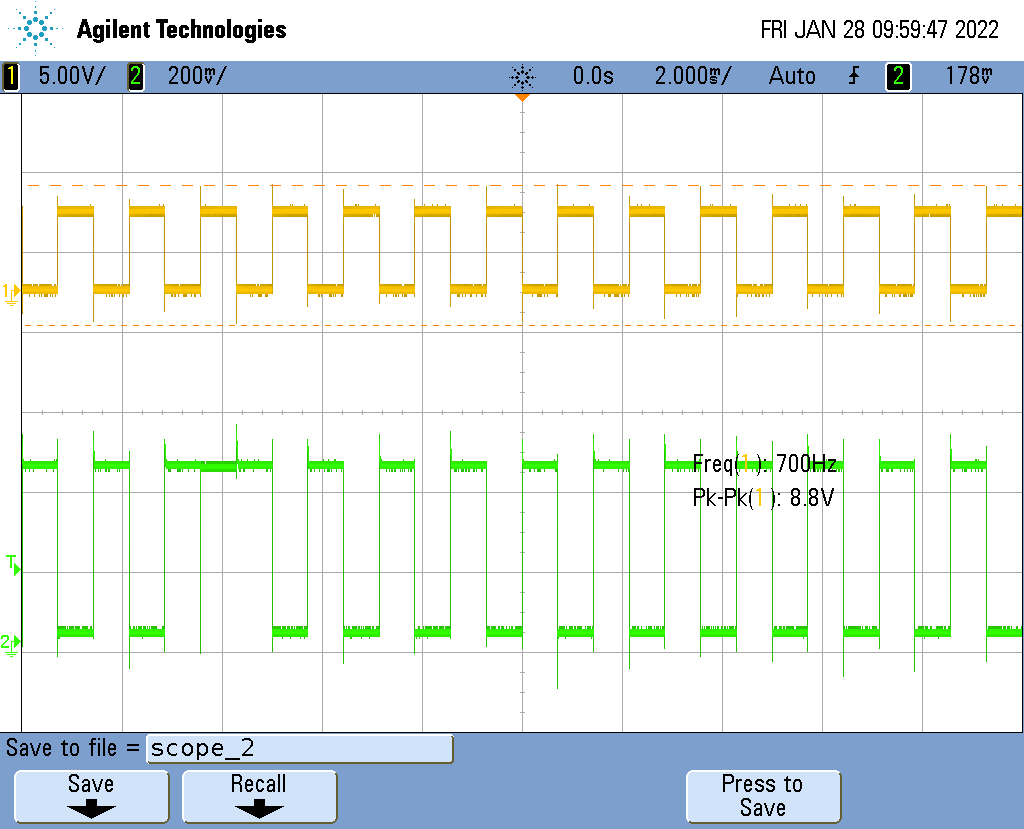
\includegraphics[width=.8\linewidth]{p1100_20k}
	  \caption{Signal at \SI{1100}{\hertz}}
	  \label{fig:sub-first}
	\end{subfigure}
	\begin{subfigure}{.5\textwidth}
	  \centering
	  % include second image
	  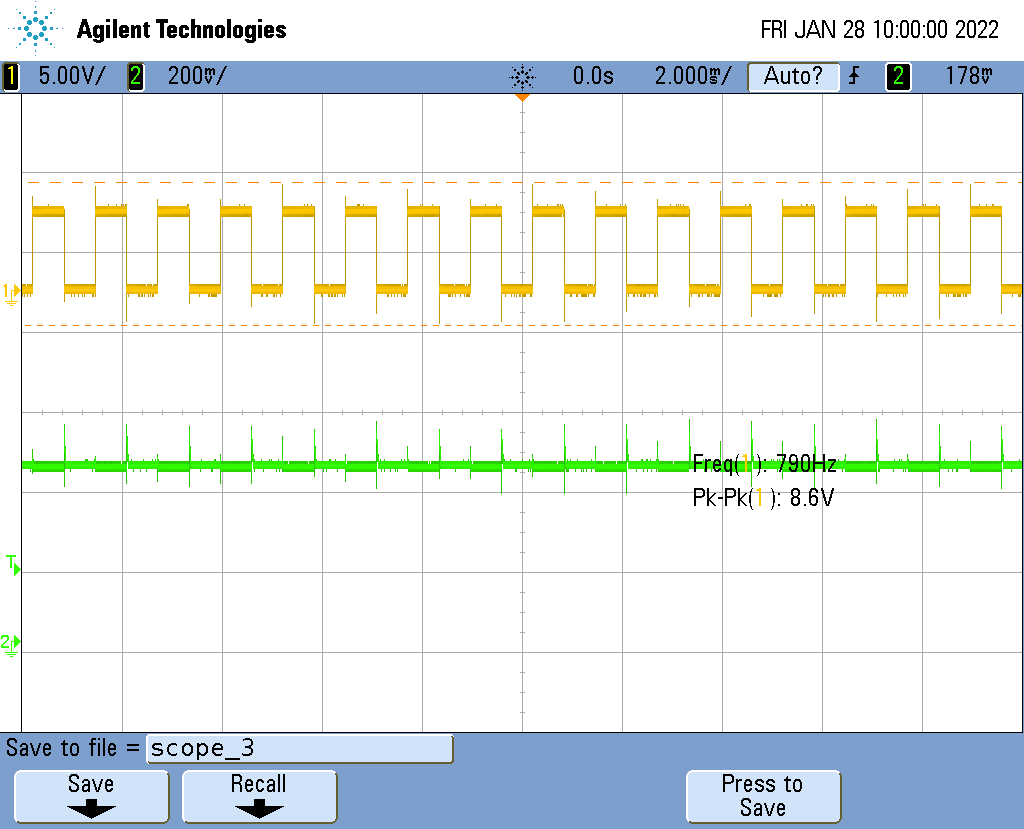
\includegraphics[width=.8\linewidth]{p1200_20k}
	  \caption{Degraded signal at \SI{1200}{\hertz}}
	  \label{fig:sub-second}
	\end{subfigure}
	\caption{Screen captures of oscilloscope with $R_L=\SI{20}{\kilo\ohm}$}
	\label{fig:p22}
	\end{figure}

	Figures \ref{fig:p21} and \ref{fig:p22} show the signal degradation experienced
	by both of the different $R_L$ values. Before signal degradation, the output
	waveform closely matched the input waveform in frequency. When the frequency of
	the input reached a critical point, the sensor seemed to output a constant
	voltage. This is due to the fact that the light being emitted by the diode
	is integrated. As the pulse reaches a critical frequency, the light integrate to
	a constant current draw from the transducer.

    \section*{Conclusion}
    This laboratory exercise constructed an optoisolator circuit which could be used
    to chart the eletrical characteristics of the OPB745 sensor. The expected behaviour
    was seen both of the tests performed. The current response of the sensor at varying
    distances could be observed and matched the expected results on the datasheet.
    The square wave input caused signal degredation at the expected frequencies noted
    in Part 2 of this exercise. Overall, this exercise was a success as the proper
    electrical characteristics of the designed circuit could be seen when tested
    experimentally.

	\section*{Questions}

	\begin{enumerate}
	\item
	A 7406 inverter will provide high impedance instead of a high logic signal. On
	the output node this would cause the low logic level to stay at zero but cause
	the high output signal to be disconnected from the circuit. This half of the
	output waveform would simply be as if the probe was not connected to a node.
	\item
	The voltage on the output starts at \SI{5}{\volt} at \SI{0}{\milli\metre} because the
	reflector is blocking the light from the emitter. This causes none of the light to
	reach the transducer on the other end of the sensor. When no light enters the
	transducer, it will not pass any current and therefore not apply a voltage drop
	across $R_L$ and therefore leaving it at \SI{5}{\volt}. The reason the voltage will
	eventually reach \SI{5}{\volt} again is because less and less light will reach the
	transducer as the distance to the reflector increases.  
	\item
	The degredation frequency increases when the load resistor is increases from
	\SI{10}{\kilo\ohm} to \SI{20}{\kilo\ohm} because the transducer will integrate
	the current it sinks. When the load resistance increases, less current is drawn
	through the load branch of the circuit and therefore shorter pulses will not
	be integrated together into a single constant output signal. I'd therefore
	anticipate the frequency to increase as the resistance increases. 
	\end{enumerate}
	
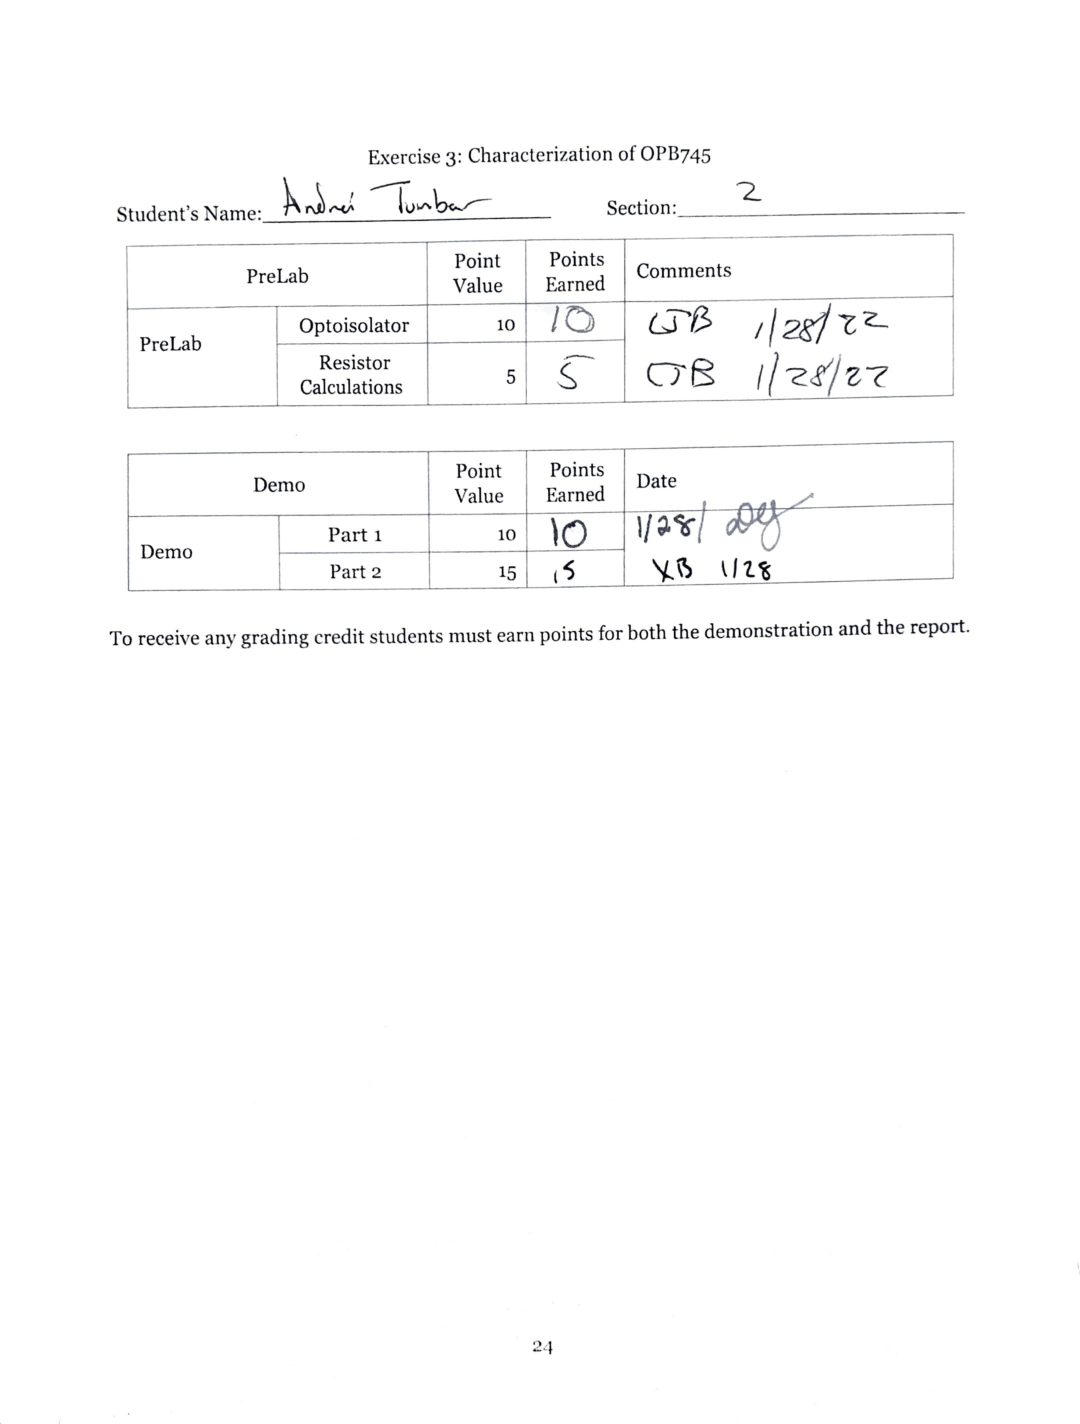
\includepdf[pages=-,pagecommand={},width=\textwidth]{signoff3.pdf}

\end{document}